\chapter{异常}

\section{异常}

\subsection{异常(Exception)}

异常就是程序在运行过程中出现的非正常的情况,它可以被捕获并处理,以防止程序崩溃。\\

Exception是一个异常类,发生异常的时候会抛出一个异常对象。如果不处理异常,程序就会被中断。\\

\begin{table}[H]
    \centering
    \setlength{\tabcolsep}{5mm}{
        \begin{tabular}{|l|l|}
            \hline
            \textbf{异常}                  & \textbf{描述}              \\
            \hline
            ArithmeticException            & 异常的运算条件             \\
            \hline
            ArrayIndexOutOfBoundsException & 非法索引访问数组           \\
            \hline
            ClassCastException             & 不匹配的类型转换           \\
            \hline
            ClassNotFoundException         & 找不到相应类               \\
            \hline
            FileNotFoundException          & 文件无法找到               \\
            \hline
            IllegalArgumentException       & 非法参数                   \\
            \hline
            IndexOutOfBoundsException      & 索引超出范围               \\
            \hline
            InputMismatchException         & 输入类型不匹配             \\
            \hline
            NullPointerException           & 空指针异常                 \\
            \hline
            NumberFormatException          & 无法将字符串转换为数字类型 \\
            \hline
        \end{tabular}
    }
    \caption{常用异常}
\end{table}

例如当数组访问越界时,会抛出一个ArrayIndexOutOfBoundsException异常;当访问一个不存在的对象时,会抛出一个NullPointerException异常。\\

\subsection{捕获异常}

try-catch-finally结构可以用于捕获并处理异常,将可能出现异常的代码放在try结构中,将异常处理的代码放在catch结构中,finally结构中的代码无论是否出现异常都会执行。\\

当在try结构中出现异常时,程序会跳转到catch结构中,执行catch结构中的代码。一个异常被处理后,将不再影响程序的执行。\\

\begin{figure}[H]
    \centering
    
\includegraphics{img/Chapter7/7-1/1.png}
\end{figure}

\mybox{整除}

\begin{lstlisting}[language=Java]
import java.util.InputMismatchException;
import java.util.Scanner;

public class Division {
    public static void main(String[] args) {
        Scanner scanner = new Scanner(System.in);

        while (true) {
            try {
                System.out.print("Enter an integer for dividend: ");
                int dividend = scanner.nextInt();
                System.out.print("Enter an integer for divisor: ");
                int divisor = scanner.nextInt();
                int quotient = dividend / divisor;
                System.out.println(
                        dividend + " / " + divisor + " = " + quotient
                );
            } catch (InputMismatchException e) {
                System.out.println("Only integers supported.");
            } catch (ArithmeticException e) {
                System.out.println("Divisor cannot be 0.");
            } finally {
                scanner.nextLine();
            }
        }
    }
}
\end{lstlisting}

\begin{tcolorbox}
    \mybox{运行结果}
    \begin{verbatim}
Enter an integer for dividend: 21
Enter an integer for divisor: 4
21 / 4 = 5
Enter an integer for dividend: 5
Enter an integer for divisor: 0
Divisor cannot be 0.
Enter an integer for dividend: 3.6
Only integers supported.
	\end{verbatim}
\end{tcolorbox}

\newpage

\section{throw与throws}

\subsection{throw / throws}

throw关键字用于抛出一个异常,一般用于程序出现某种逻辑时程序员主动抛出某种特定类型的异常。\\

throws关键字用在声明方法的时候,表示该方法可能要抛出异常。定义了throws异常抛出类型的方法,在当前的方法中可以不处理这个异常,由调用方处理。\\

\begin{figure}[H]
    \centering
    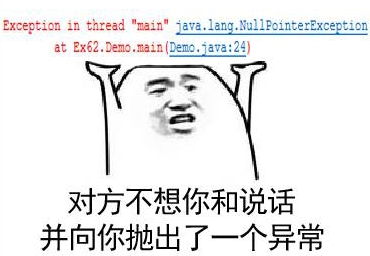
\includegraphics{img/Chapter7/7-2/1.png}
\end{figure}

\mybox{抛出异常}

\begin{lstlisting}[language=Java]
public class Person {
    private int age;
    
    public void setAge(int age) throws Exception {
        if(age < 0 || age > 130) {
            throw new Exception();
        }
        this.age = age; 
    }
    
    public static void main(String[] args) {
        try {
            Person person = new Person();
            person.setAge(-1);
        } catch(Exception e) {
            System.out.println("年龄异常");
        }
    }
}
\end{lstlisting}

\begin{tcolorbox}
    \mybox{运行结果}
    \begin{verbatim}
年龄异常
	\end{verbatim}
\end{tcolorbox}

\newpage

\section{自定义异常}

\subsection{自定义异常}

使用异常是为了处理一些重大的逻辑bug,这些逻辑bug可能会导致程序的崩溃。此时,可以使用异常机制,强迫修改这个bug。\\

系统中提供了很多的异常类型,但是异常类型提供地再多,也无法满足所有的需求。当需要的异常类型系统没有提供的时候,此时就需要自定义异常了。\\

系统提供的每一种异常都是一个类,所以自定义异常其实就是写一个自定义的异常类。自定义的异常类,理论上来讲,类名可以任意定义,但是出于规范,一般都会以Exception作为结尾,例如ArrayIndexOutOfBoundsException、NullPointerException、ArithmeticException等。\\

如果要自定义一个编译时异常,需要继承自Exception类,如果要自定义一个运行时异常,需要继承自RuntimeException类。\\

\mybox{自定义异常}

\begin{lstlisting}[language=Java]
public class AgeException extends RuntimeException {
    public AgeException() {
        super("年龄异常");
    }
    
    public AgeException(int age) {
        super("年龄异常:" + age);
    }
}
\end{lstlisting}

\begin{lstlisting}[language=Java]
public class Person {
    private int age;
    
    public void setAge(int age) throws AgeException {
        if(age < 0 || age > 130) {
            throw new AgeException(age);
        }
        this.age = age;
    }
    
    public static void main(String[] args) {
        try {
            Person person = new Person();
            person.setAge(-1);
        } catch(AgeException e) {
            e.printStackTrace();
        }
    }
}
\end{lstlisting}

\begin{tcolorbox}
    \mybox{运行结果}
    \begin{verbatim}
AgeException: 年龄异常:-1
at Person.setAge(Person.java:6)
at Person.main(Person.java:15)
	\end{verbatim}
\end{tcolorbox}

\newpage